\documentclass[11pt,a4paper]{scrartcl}
\usepackage[czech]{babel}
\usepackage[utf8]{inputenc}
\usepackage{graphicx}
\usepackage{float}
\graphicspath{{./img/}}

\begin{document}
	\begin{figure}[h!]
		\centering
		
\includegraphics[bb= 0 0 820 445 , width=75mm]{favlogo.jpg}
	\end{figure}
	
	\vspace{5cm}
	
	{\centering
		{\huge KIV/OS - Semestrální práce}\\[1em]
		{\large Simulátor operačního systému}\\[7,5cm]
	}
	
	\begin{center}
		\begin{tabular}{l l}
		autoři: & Daniel HRYZBIL (A19N0076P), \\
		& Anežka JÁCHYMOVÁ (A19N0077P), \\
		& Zdeněk VALEŠ (A17N0094P) \\
		datum: & 29.11.2019 \\
		\end{tabular}
	\end{center}
	
	\thispagestyle{empty}
	\newpage
	
	\section{Zadání}
	\begin{enumerate}
		\item 	Vytvořte virtuální stroj, který bude simulovat OS
		\item 	Součástí bude shell s gramatikou cmd, tj. včetně exit
		\item 	Vytvoříte ekvivalenty standardních příkazů a programů:
		\begin{enumerate}
			\item echo, cd, dir, md, rd, type, find /v /c"" (tj. co dělá wc v unix-like prostředí), sort, tasklist, shutdown
			
			\begin{itemize}
				\item	cd musí umět relativní cesty
				\item	echo musí umět @echo on a off
				\item	type musí umět vypsat jak stdin, tak musí umět vypsat soubor
			\end{itemize}
		
			\item	Dále vytvoříte programy rgen a freq
			\item	rgen bude vypisovat náhodně vygenerovaná čísla v plovoucí čárce na stdout, dokud mu nepřijde znak Ctrl+Z //EOF
			\item	freq bude číst z stdin a sestaví frekvenční tabulku bytů, kterou pak vypíše pro všechny byty s frekvencí větší než 0 ve formátu: “0x\%hhx : \%d”
		\end{enumerate}
		\item 	Implementujte roury a přesměrování
		\item 	Nebudete přistupovat na souborový systém, ale použijete simulovaný disk
		
		\begin{itemize}
			\item 	Za 5 bonusových bodů můžete k realizaci souborového systému použít semestrální práci z KIV/ZOS - tj. implementace FAT.
		\end{itemize}
	\end{enumerate}

	\section{Kernel}
	Jádro poskytuje API pro správu procesů a vláken, vytvoření pipe a přístup k disku, ke kterému je možné z user space přistoupit systémovým voláním.
	
	\subsection{Handle}
	
	Základním konceptem kernelu je třída \verb|HandleStorage| společně s \verb|HandleReference|. Každá třída reprezentující nějaký handle (soubor, proces, vlákno, ...) implementuje rozhraní \verb|IHandle|. Všechny instance těchto tříd jsou následně uloženy uvnitř \verb|HandleStorage|, kde jim je přiřazeno jejich unikátní \verb|HandleID| (16 bitové číslo). Toto číslo se také předává do user-space jako indentifikátor daného handle. Přístup k uloženým handle je následně možný pouze přes objekty \verb|HandleReference|. Struktura handlů je znázorněna diagramem tříd na obrázku \ref{fig:handle-class-d}.
	
	\begin{figure}[H]
		\centering
		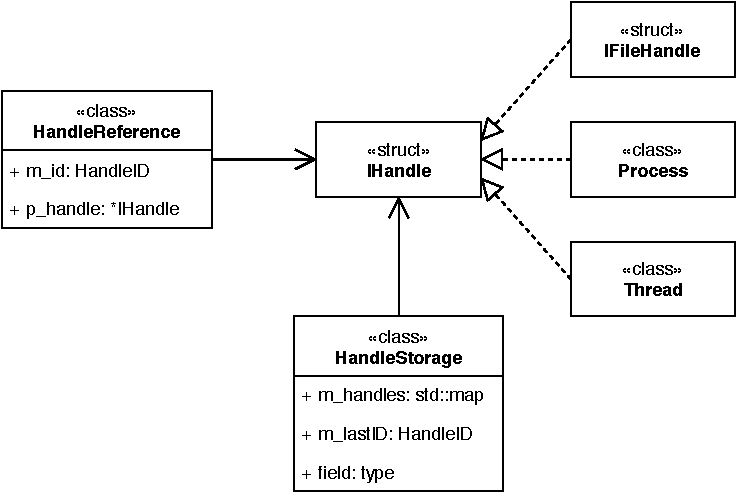
\includegraphics[width=11cm]{handle-class-d.pdf}
		\caption{Diagram tříd handle}
		\label{fig:handle-class-d}
	\end{figure}
	
	Uvnitř \verb|HandleStorage| je pro každý handle uložen počet referencí na tento handle, který se inkrementuje vždy při vytvoření nové \verb|HandleReference| a dekrementuje při odstranění \verb|HandleReference|. Handly s nulovým počtem referencí jsou automaticky uzavřeny a odstraněny ze systému. 
	
	Každý proces si udržuje vlastní množinu referencí na handly, které byly v jeho kontextu vytvořeny nebo jinak získány (například při vytváření procesu předá rodičovský proces nově vytvořenému procesu handle na \verb|stdin| a \verb|stdout|). Tato množina se zároveň používá i pro zjištění, zda má proces k nějakému handlu vůbec přístup. Při odstranění procesu potom dojde k odstranění všech handle referencí uložených v jeho množině, a tím dojde automaticky i k odstranění všech handlů, které používal pouze daný proces. 
	
	Kernel se tak nespoléhá na \uv{slušnost} user-space kódu, který by měl vždy použít \verb|CloseHandle|, ale dokáže při ukončení procesu automaticky uklidit všechny nepotřebné handly stejně jako reálný OS. Zároveň tento koncept umožňuje i efektivnější spolupráci více vláken najednou. Při práci s nějakým handle totiž není potřeba zamykat globální zámky, protože pokud pro tento handle existuje alespoň jeden objekt \verb|HandleReference|, tak je zaručeno, že žádné jiné vlákno nemůže tento handle nečekaně odstranit a způsobit tak pád celého systému.
	
	\subsection{Procesy a vlákna}
	
	Procesy jsou uloženy v již zmíněném \verb|HandleStorage| a \verb|HandleID| je bráno jako PID. Stejně tak jsou uložena i vlákna a \verb|HandleID| představuje TID. Každé vlákno simulovaného OS využívá reálné vlákno fyzického OS (\verb|std::thread|). Za hlavní vlákno procesu se považuje jeho první vlákno. Při vytvoření procesu je vždy vytvořeno i jeho hlavní vlákno.
	
	\subsubsection{API}
	Procesy a vlákna jsou reprezentovány handly, API pro práci s nimi tedy očekává (případně vrací) patřičný handle.
	
	\paragraph{Create Process}
	Vytvoří nový proces.
	
	\begin{figure}[H]
		\centering
		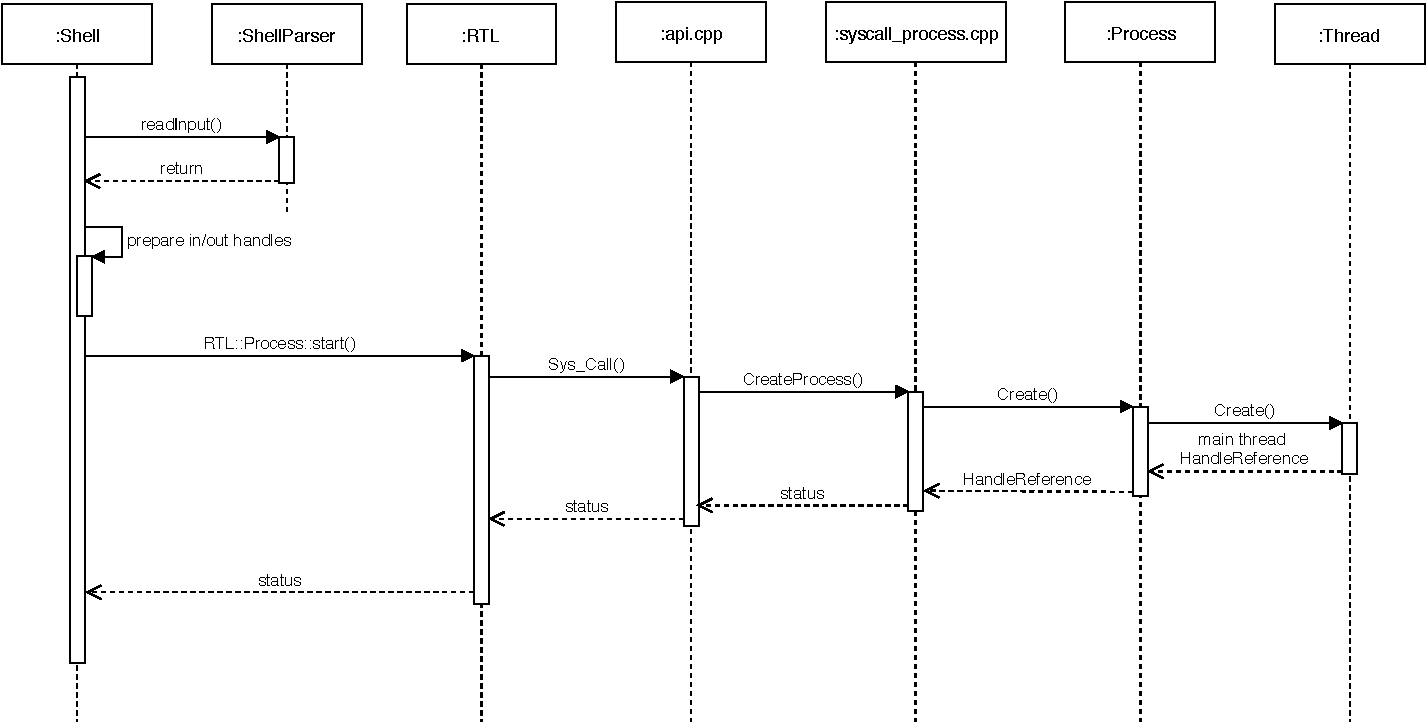
\includegraphics[width=14cm]{create-process-seq.pdf}
		\caption{Sekvenční diagram vytvoření procesu}
		\label{fig:create-process-seq}
	\end{figure}
	
	\paragraph{Create Thread}
	Vytvoří nové vlákno v kontextu aktuálního procesu.
	
	\paragraph{Wait For}
	Počká, až se zadané procesy nebo vlákna ukončí.
	
	\begin{figure}[H]
		\centering
		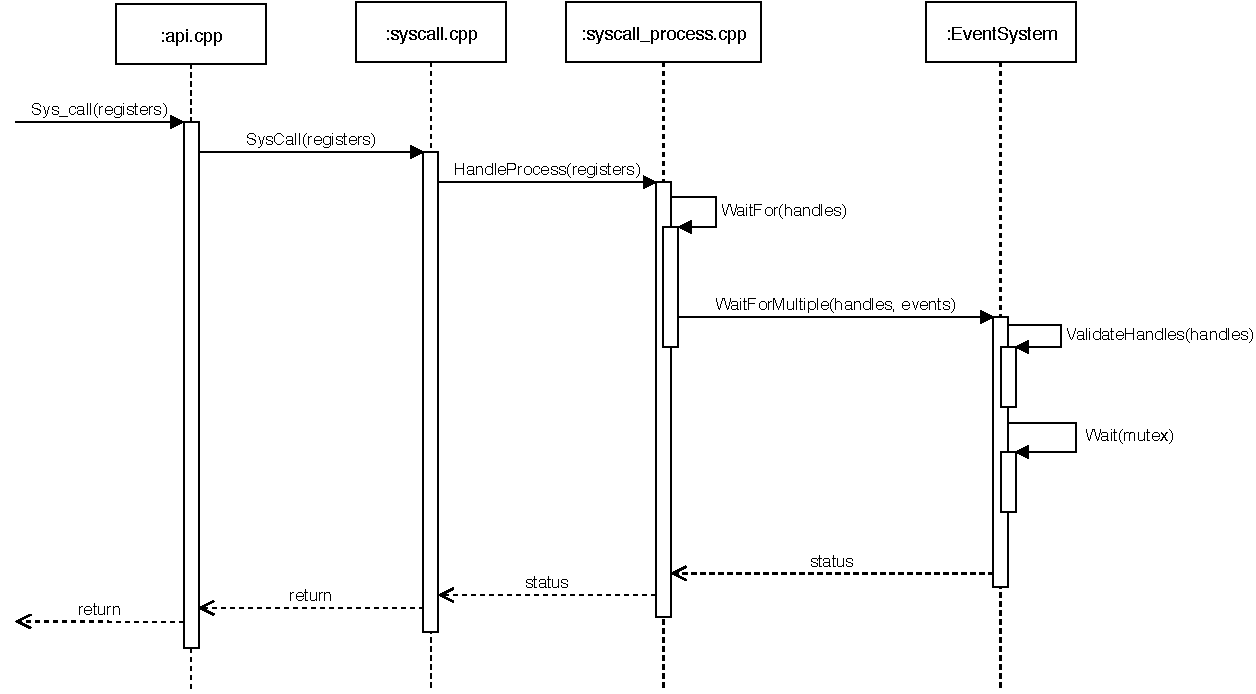
\includegraphics[width=14cm]{wait-for-proc.pdf}
		\caption{Sekvenční diagram čekání na vlákno nebo proces}
		\label{fig:wait-for-proc}
	\end{figure}
	
	\paragraph{Get Exit Code}
	Získá návratový kód procesu nebo vlákna.
	
	\paragraph{Setup Signal}
	Nastaví signal handler. Signály se posílají vždy vláknům. Každé vlákno má svůj signal handler a seznam signálů (signal mask), které se mohou doručit tomuto handleru. Pro jednoduchost má každé vlákno pouze jeden signal handler společný pro všechny signály (v OS je definovaný stejně jen jeden signál). Při každém vstupu vlákna do jádra (syscall) se zkontroluje, zda nebyl danému vláknu odeslán nějaký signál, a pokud ano, tak se spustí jeho signal handler (pokud nějaký má a pokud je daný signál v seznamu signálů, které se mohou doručit). Stejná kontrola se provádí i při výstupu vlákna z jádra (konec syscallu). To kvůli delšímu blokování vlákna v jádře (například čekání na vstup od uživatele nebo čekání na ukončení jiného procesu nebo vlákna). Signal handler se tak spouští vždy v kontextu vlákna, ve kterém byl nastaven.
	
	\paragraph{Exit}
	Nastaví návratový kód aktuálního vlákna. Samotné ukončení musí vlákno provést samo návratem ze své vstupní funkce. Standardní knihovna C++ ani neposkytuje žádný způsob, jak ukončit běžící vlákno (\verb|std::thread|). Bylo by sice možné použít platform-specific funkce z WinAPI (\verb|ExitThread| nebo \verb|TerminateThread|), ale násilné ukončení běžícího vlákna představuje z pohledu jazyka C++ velký problém, protože se nemusejí zavolat všechny destruktory a nedojde tak k uvolnění všech zdrojů alokovaných v daném vlákně. Z tohoto důvodu se vlákno musí vždy ukončit samo, což by v reálném OS nebylo moc dobré. Návratový kód procesu je vždy návratový kód hlavního vlákna daného procesu. Proces se považuje za ukončený, pokud už neobsahuje žádná běžící vlákna.
	
	\paragraph{System Shutdown}
	Uzavře všechny souborové handly a pošle signál \verb|Terminate| všem aktivním vláknům v systému.

	
	\subsection{Filesystem}
	
	Kernel obsahuje file system manager, který spravuje disky a souborové systémy na nich uložené. Pro přístup na disk je použito abstraktní API (\verb|IFileSystem|), které implementuje každý ovladač pro FS. Struktura je znázorněna na obrázku \ref{fig:fs-layers}.
	
	\begin{figure}[H]
		\centering
		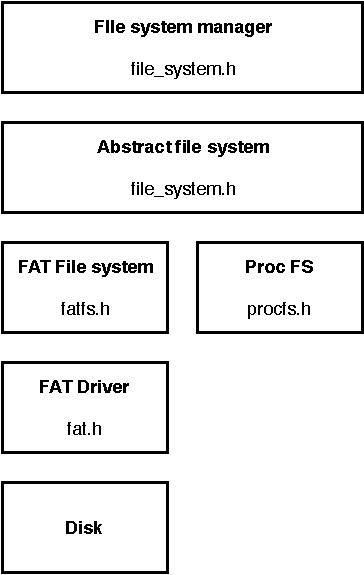
\includegraphics[height=9cm]{fs-layers.pdf}
		\caption{Struktura správy souborových systémů}
		\label{fig:fs-layers}
	\end{figure}

	\paragraph{Soubory} Každý souborový handle implementuje rozhraní \verb|IFileHandle|. Handly otevřených souborů a adresářů jsou uloženy ve výše zmíněném \verb|HandleStorage|. Otevřený soubor nebo adresář je reprezentován objektem třídy \verb|File|, která také implementuje \verb|IFileHandle|. K synchronizaci přístupu více vlákny je použit mutex (\verb|std::mutex|). Struktura handlu je znázorněna na obrázku \ref{fig:file-handler}.
	
	\begin{figure}[H]
		\centering
		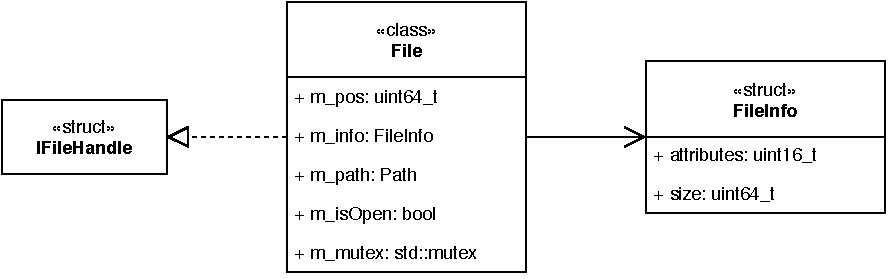
\includegraphics[width=11cm]{file-handler.pdf}
		\caption{Struktura souborového handle}
		\label{fig:file-handler}
	\end{figure} 
	
	\subsubsection{API}
	K datům každého souborového systému je přistupováno skrze API definované v \verb|IFileSystem|. Uživatelská vrstva pak k API přistupuje skrze systémová volání.
	
	\paragraph{Create}
	Vytvoří soubor nebo adresář.
	
	\paragraph{Query}
	Získá informace o souboru nebo adresáři.
	
	\paragraph{Read}
	Přečte soubor (nebo jeho část) do bufferu. Offset od kterého se čte je získán z handle souboru.
	
	\paragraph{ReadDir}
	Načte soubory v adresáři.
	
	\paragraph{Remove}
	Odstraní soubor nebo prázdný adresář.
	
	\paragraph{Resize}
	Změní velikost souboru.
	
	\paragraph{Write}
	Zapíše data do souboru. Offset od kterého se zapisuje je získán z handle souboru.
	
	
	\subsubsection{FAT}
	
	Jako hlavní souborový systém jsme zvolili FAT implementovanou v rámci KIV/ZOS. Rozložení souborového systému na disku je znázorněno na obrázku \ref{fig:fat-disk-struct}. V původní specifikaci je na disku uložena alespoň jedna další kopie FAT tabulky, která se používá ke kontrole bloků dat. Protože kontrolu poškozených dat v práci neprovádíme, rozhodli jsme se ukládat pouze jednu kopii.
	
	\begin{figure}[H]
		\centering
		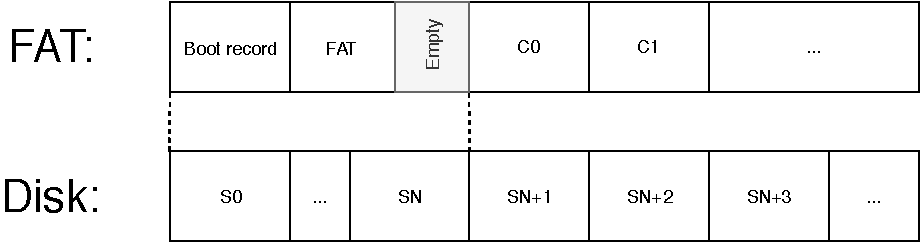
\includegraphics[width=12cm]{fat-rozdeleni-disku.pdf}
		\caption{Uložení FAT souborového systému na disk}
		\label{fig:fat-disk-struct}
	\end{figure}

	Velikost jednoho datového clusteru je dána velikostí sektorů na disku a platí, že 1 cluster = N $\times$ sektor, kde $N$ je vypočítané při inicializaci souborového systému na disku. Root adresář začíná na clusteru 0. Metadata každého souboru jsou reprezentována strukturou \verb|Directory| (obrázek \ref{fig:dir-c}). Adresáře jsou od souborů odlišeny nastaveným bitem ve \verb|flags|. Jméno souboru může být maximálně 11 znaků (12. znak je \verb|'\0'|).
	
	\begin{figure}[H]
		\centering
		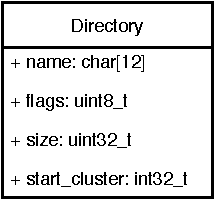
\includegraphics[width=3cm]{dir-c.pdf}
		\caption{Struktura Directory}
		\label{fig:dir-c}
	\end{figure}


	\subsubsection{ProcFS}
	\label{sec:proc-fs}
	Přístup k aktuálně běžícím procesům je realizován přes virtuální souborový systém, který je mapován na disk \verb|0:\|. Struktura je znázorněna na \ref{fig:procfs-struct}. V kořenovém adresáři existuje pro každý běžící proces adresář pojmenovaný podle \verb|HandleID| daného procesu. Dále je zde adresář \verb|self|, který vždy odkazuje na aktuální proces. Adresáře jednotlivých procesů obsahují popisné soubory, ze kterých je možné přečíst informace o daném procesu:
	
	\begin{itemize}
		\item Název programu
		\item Parametry se kterými byl proces spuštěn
		\item Aktuální pracovní adresář
		\item Počet běžících vláken
	\end{itemize}
	
	\begin{figure}[H]
		\centering
		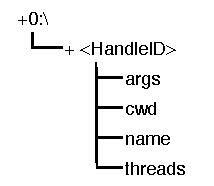
\includegraphics[width=3cm]{procfs-struct.pdf}
		\caption{Struktura ProcFS}
		\label{fig:procfs-struct}
	\end{figure}
	
	\verb|ProcFS| také dědí od \verb|IFileSystem| a implementuje tedy kompletní API pro přístup k datům. Celý \verb|ProcFS| je ale pouze pro čtení, takže všechny funkce kromě \verb|query()|, \verb|read()| a \verb|readDir()| vždy vrací chybu \verb|PERMISSION_DENIED|. K vypsání všech běžících procesů lze použít funkci \verb|readDir(0:\)|.
	
	Detaily libovolného procesu je možné získat voláním \verb|read(0:\<HandleID>\<proc_file_name>)|. Místo \verb|HandleID| lze použít \verb|self|, API pak vrací detaily o aktuálně běžícím procesu.

	
	\subsection{Roura}
	
	Roura je tvořena dvěma propojenými handly - \verb|PipeReadEnd| a \verb|PipeWriteEnd| (viz obrázek \ref{fig:pipe-c}). Čtecí konec obsahuje buffer, do kterého se zapisuje ze zapisovacího konce. Při uzavření jednoho konce se spojení mezi nimi přeruší a druhý konec tak ví, že už při prázdném bufferu nemá čekat na další data (čtecí konec) nebo při plném bufferu čekat na uvolnění místa (zapisovací konec).
	
	\begin{figure}[H]
		\centering
		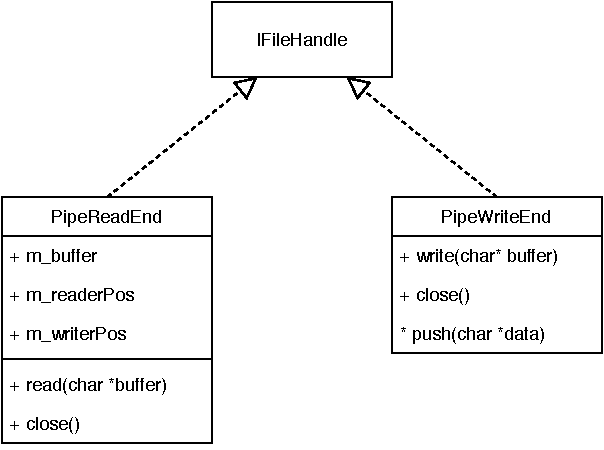
\includegraphics[width=8cm]{pipe-c.pdf}
		\caption{Pipe diagram tříd}
		\label{fig:pipe-c}
	\end{figure}
	
	\section{RTL}
	Runtime knihovna obaluje systémová volání a umožňuje tak pohodlnou komunikaci user-space programů s jádrem. Obsahuje také obalové třídy reprezentující proces, vlákno, soubor, adresář a rouru. Celá se nachází v \verb|rtl.h| a \verb|rtl.cpp|.
	
	\section{Shell a uživatelské příkazy}
	Proces shellu je spuštěn po startu systému. Shell ve smyčce čte po řádcích ze standardního vstupu, řádky parsuje a spouští rozparsované příkazy. Pokud shell obdrží signál \verb|Terminate|, smyčka je ukončena a shell se vypne.
	
	\subsection{Parser}
	Implementován třídou \verb|ShellParser| v \verb|shell.cpp|. Z rozparsované řádky vrátí strukturu obsahující příkazy, které se mají vykonat a informace o případném přesměrování (\verb|<|, \verb|>|, \verb|>>|). Přesměrování \verb|>| nastaví velikost cílového souboru na 0 a pak do něj od začátku zapisuje. Přesměrování \verb|>>| nastaví pozici cílového souboru na jeho konec a pak za něj zapisuje data.
	
	\subsection{Implementace příkazů}
	Každý příkaz je shellem spouštěn jako samostatný proces. Před spuštěním shell procesu nastaví handly na standardní vstup a výstup. Kód příkazu pak volá funkce RTL pro čtení ze standardního vstupu a zápis do standardního výstupu. RTL si z kontextu aktuálně běžícího vlákna sama získá handly standardního vstupu a výstupu daného procesu, takže získání a uložení těchto handlů není potřeba řešit v kódu každého programu.
	
	\paragraph{dir}
	Vypíše na výstup seznam souborů v zadaném adresáři. Cest lze příkazu skrze parametry předat více. Příkaz otevře zadaný adresář funkcí \verb|RTL::OpenDirectory(path)|. Obsah adresáře je získán funkcí \verb|RTL::GetDirectoryContent(dirHandle)|.
	
	\paragraph{echo}
	Vypíše text ze vstupu na výstup. Echo lze vypnout příkazem \verb|@echo off| (a zapnout \verb|@echo on|). Proměnná, která drží stav echa je uložena v každé instanci shellu zvlášť. K výpisu na výstup je použita funkce \verb|RTL::WriteStdOut()|.
	
	\paragraph{find}
	Podporujeme pouze příkaz \verb|find /C /V ""|, tj. s prázdným řetězcem k vyhledání. Příkaz čte po řádcích text ze vstupu dokud nepřijde EOF. Pak vypíše počet zadaných řádek.
	Význam přepínačů: 
	\begin{itemize}
		\item  \verb|/C| Počet řádek, které text obsahují,
		\item \verb|/V| Zobrazí řádky, které zadaný text neobsahují.
	\end{itemize}
	
	
	\paragraph{freq}
	Čte vstup dokud nepřijde EOF a udělá statistiku, kolikrát byl který byte na vstupu přítomen. Po dokončení statistiky je výsledek vypsán na výstup. 
	
	\paragraph{md}
	Vytvoří zadaný adresář. Adresářů lze skrze parametry předat více. Příkaz vytvoří adresář voláním funkce \verb|RTL::CreateDirectory(path)|.
	
	\paragraph{rd}
	Smaže zadaný soubor. Použitím parametru \verb|/S| lze rekurzivně mazat adresářové stromy. Soubor je smazán voláním funkce \verb|RTL::DeleteDirectory(path)|.
	
	\paragraph{rgen}
	Generuje náhodná čísla v rozmezí $<0;1)$, která vypisuje na výstup. Čísla jsou generována dokud na vstupu není EOF.
	
	\paragraph{shutdown}
	Vypne systém voláním funkce \verb|RTL::Shutdown()|.
	
	\paragraph{sort}
	Čte řádky ze vstupu a řadí je. Po přečtení EOF vypíše seřazené řádky na výstup.
	
	\paragraph{tasklist}
	Zavolá \verb|OpenDirectory("0:")| čímž otevře virtuální disk 0 (viz sekce \ref{sec:proc-fs}), načte jeho obsah (\verb|GetDirectoryContent()|) a vypíše jej na výstup.
	
	\paragraph{type}
	Vypíše na výstup obsah zadaných souborů. K otevření souboru je použita funkce \verb|RTL::OpenFile(path)|, k získání obsahu pak \verb|RTL::ReadFile(handle, buffer)|.
	
\end{document}
